\newpage
\section{Discussion} \label{Discussion}

\begin{comment}
the discussion, in which you connect the results to the research questions and the literature

aanpak log verwerking:
- totaliseren van de results
- actie research: wat ben ik aan het doen
- experimenteren in de praktijk
- deel uitmaken van het proces
- laten gebeuren
- valt me op dat .... -> content analyse
- cluster waarneming -> beschouwen: het valt me op dat .. en onderbouwing
- bottom up (logs) en top down (gesprekken)
- bij elk log -> wie wat waar; traceerbaar houden







TODO


=======
- iemand moet het nalezen op consistentie
- nalezen op vorm
- checken of de referenties nog kloppen


- hoe ga je straks om met wijzigingen in de wet. 
- Vanuit de wet weet je straks wat de wijzingen zijn, maar ga je deze ook in scripts terugvinden.



H5 -> observaties kritisch  bekijken -> welke zaken komen vaak voor
\end{comment}
The most common keywords within the observations in appendix ~\ref{appendixLoglines}, in table~\ref{tab:table-totalCounts} on page~\pageref{tab:table-totalCounts} are with the terms "Ampersand", "Api ","Concept", "Conceptual analysis",
"Interface", "Law", "Multiplicity", "Relation" and "Rule".
These are terms that in most cases are part of the Amersand method.
Only the term "law" refers to the case itself.

This chapter focuses on the relationship between the results (see section~\ref{Results} and the sub-questions.

\subsection{Ampersand knowledge}\label{subsection:ampersand-knowledge}
When working with Ampersand, a development environment must first be set up.
Ampersand's documentation assumes that XAMPP~\footnote{\url{https://github.com/AmpersandTarski/documentation/blob/master/installing-ampersand/installing-the-tools-manually.md}} can be configured for this become.
The preferred configuration is done with the help of Docker.
If there is little or no knowledge of Docker, you can choose to set up XAMPP.
However, it was not possible to get the local installation working with the help of the documentation.
However, with help we managed to get it working in the Docker environment.
So starting with Ampersand, it's not just Ampersand that needs to be studied, it's also the environment in which it operates that needs to be studied.
This part always works.
Setting up the environment and Ampersand is also fine from the website and from github.
There is also some information on stackoverflow.
But beyond that there is nothing to be found outside of a number of scientific articles.
Fortunately, there are articles like \cite{de_swart_ampersand_2011} that explain Ampersand.

The sub-question "\acrlong{RQ1}" examines the knowledge of the software engineer when using Ampersand.

In order to be able to use Ampersand itself, in addition to knowledge about the structure of the environment, knowledge of Ampersand itself is required.
There is not a lot of information about Ampersand on the internet.
And there are examples, but they do not cover the whole load.
As with any tool and method, knowledge will have to be kept up to date to keep Ampersand usable.
This is not specific to Ampersand, but of course also applies to Ampersand.

Proper use of Ampersand requires proper documentation setup.
This setup consists of knowledge of the way Ampersand handles the information in the scripts.
The positioning of the meaning of the Terms and the Relationships and the purpose of the Rule and the use of includes.
One should be aware that the meaning, purpose and definitions appear directly in the documentation and the inclusions help determine the order of the story and that this should be a unifying story.
Agreement must be reached in advance about the structure of the spelling, the reference to legislation and regulations.
The notation method, the naming convention of Concepts and Relations must also be unambiguous in order to have a consistent and professional appearance.
And, as one of the interviewees pointed out, when documentation needs to be done, why not through Ampersand.
Unfortunately, the researcher started to standardize somewhat later, so that this was not implemented everywhere.

When working with Ampersand and going through the text, it seems logical to go through the text chronologically.
However, this will not always work and a method must be found to maintain the overview.
This is very difficult when using Ampersand because Ampersand is so close to processing the original source text.
This aspect has been approached in various ways.
The source text in XML has been looked at, with the intention of adding extra XML tags.
The intended side effect of this was that we could generate the model from the XML.
This didn't work because the original XML is way too complex and would make the XML parsing very complex as well.
And the work has to be redone with a new version of the law.
The RTF format was like a Word document and could be provided with comments.
The same was true for the PDF format.
Annotation is also possible here and one can also underline with colors.
In the end, the old-fashioned choice was made for the combination of hard copy and the PDF.
Hard copy for streaking and writing and the PDF for searching and copying text.

Maintaining the overview in the created scripts is also a challenge.
By using Visual Studio there are no refactor options.
Visual Studio also seems to lack integration between the scripts.
The consequence of this is that it is possible that the same Concepts and also Relationships are defined in several places.
By not being aware of the overlap, a different definition can occur for the same Concept.
The differences will not be very large, but certainly worded differently.
This only came to light when the documentation was generated.
The advantage of working with text and generating the model from it appears to be a disadvantage here.

Article 3(1) of the \acrshort{big} states that there are several registers.
In order to implement this, an attempt has been made to install a single register in combination with the shared piece.
The shared components appear in each register and include the person registration and the registration leading to the actual registration.
The implementation of the prototype of a profession with the common part was no problem.
Until the next profession was established.
Then the first professional group was removed from the database and the common data was also removed and the second group was fully initiated.
The method of building specific professional registers in this way is not (yet) supported by Ampersand.
If this does not work for this law, it will also not work for links with other registers where data and the associated management software must be shared.

Every organization has an authorization mechanism for the software.
The \acrshort{cibg} uses a JWT mechanism.
In the research I encountered an authorization mechanism when creating the Rules and when building the Interface.
I have not found out whether it is possible to integrate this with the organization's own authorization mechanism.


The team that Ampersand maintains and wants to expand is very active.
The involvement is also apparent from the rapid resolution of issues that occurred.


\subsection{Ampersand core in wet Big}\label{subsection:ampersand-core-in-wet-big}
With sub-question "\acrlong{RQ2}" we want to know what is in the \acrlong{ca}.
For this appendix~\ref{appendixContentAnalysis} is included.
The \acrlong{ca} contains the Concepts, Relations and Rules.
The \acrlong{ca} is not complete because not all articles and related regulations has been analyzed.


\subsection{Setup law for Ampersand}\label{subsection:setup-law-for-ampersand}
The sub-question "\acrlong{RQ3}" deals with the law, in the case of the \acrshort{big}, and the way in which it can be analyzed and processed using Ampersand.
Interviews paint a picture of a law that originated in the 19th century.
Although this has been adapted to the current times, the structure is not equipped for a one-to-one translation to an information system.
It has been indicated that there are new laws that are much better suited for translation, such as, for example, "Regeling bewijsstukken sociale hygiëne Drank- en Horecawet 2015".
Since we have not analyzed any other laws, it cannot be determined whether this is the case.
But the \acrshort{big} is a large and complex law, according to a lawyer at the \acrshort{cibg}.

Analyzing the law requires legal knowledge.
Reading the legal texts also requires the necessary experience.
Analyzing the law is usually not the domain of a business analyst.
At the start of the analysis, a team should be set up that should include at least an analyst and a lawyer.
The analyst for building and managing the script and the lawyer for the translation of the law into Concepts and Relationships.
This ensures consistency and completeness of the analysis.
It has been found that even a lawyer can understand the concepts and the relationships of conceptual analysis.
As a result, the cooperation on this point will run smoothly.

By starting the law with the help of a lawyer, an overview can be obtained at an early stage of the content and structure of the law.
By looking at the structure, the analyst can better understand what the law is about.
The structure can also help to determine the structure of the patterns.
It's certainly not the case that every chapter is a separate pattern, but it certainly influences the setup of the \acrlong{ca}.
And thereby help to gain an overview of the law and, on the other hand, of the analysis to be performed.


\subsection{Ampersand for registry systems}\label{subsection:ampersand-for-registry-systems}
The sub-question "\acrlong{RQ4}" focuses on the use of Ampersand within the \acrshort{cibg} organization.
The information systems that are not based on legislation and regulations and which aim to monitor data quality are often the registers.
\acrshort{cibg} builds, manages and monitors this data through registration systems.

In discussions with architecture of the CIBG, the issue of maintenance on the Ampersand model comes up.
When a model is initially set up, this results in a certain version of the model.
The model consists of a database model and the other software.
This model can be implemented.
During the life-cycle of the software, the legislation will certainly be amended.
Including these changes in the model will result in a new model.
This new model is definitely different from the old model.
Ampersand does not provide any resources to guide the conversion from the old model to the new model.
So the development team will have to make an analysis of the old and the new situation.
And have to develop conversion software for this.
This is a method that is different from usual.
Usually, when the software is changed, the changes in the database are immediately taken into account.
The advantage of a new model is that the software does not have to deal with legacy.
So it is always a state-of-the-art model.
The downside is that the conversion is likely to be complex.
Data that was previously valid could just be invalid in a subsequent model.

Ampersand is clearly not equipped to support processes.
The execution of management processes is left to the organization.
Ampersand is declarative and reactive, so the Ampersand implementation always responds to the current situation through validations.

Although Ampersand is intended as a design and prototyping tool, it does have APIs at its disposal.
This can only be obtained from log lines and apparently not intended as a means of communication from external systems.
This is also apparent from the fact that no API description is made in, for example, Swagger~\footnote{\url{https://swagger.io}}.
But it can work that way.
It is possible to communicate with the Ampersand core from an external source.
The return actions from the called APIs are not provided with a code but text.
As proof of concept, calls were made from Postman~(see figure~\ref{fig:postman-get-person}) to Ampersand and that worked as expected, see figure~\ref{list:postman-output}.
\begin{figure}[ht]
    \centering
    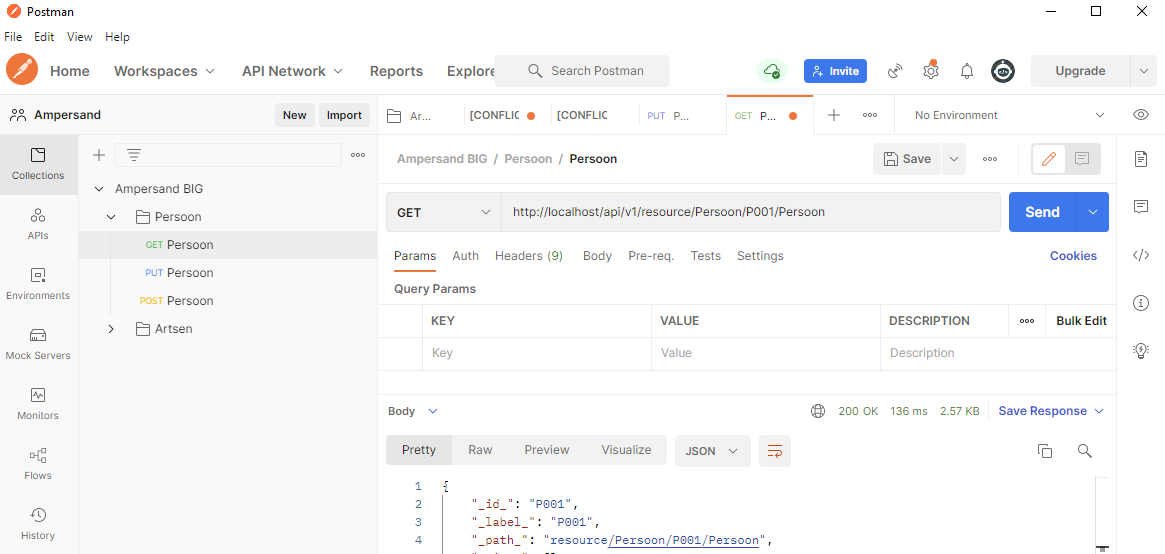
\includegraphics[width=\textwidth]{/postman_GET.PNG}
    \caption{Postman GET Person}
    \label{fig:postman-get-person}
\end{figure}

\begin{lstlisting}[language=json,firstnumber=1,caption={Postman output from GET Person},captionpos=b,label={list:postman-output}]
{
    "_id_": "P001",
    "_label_": "P001",
    "_path_": "resource/Persoon/P001/Persoon",
    "_view_": [],
    "Persoon": {
        "_id_": "P001",
        "_label_": "P001",
        "_path_": "resource/Persoon/P001/Persoon/Persoon",
        "_view_": [],
        "_ifcs_": []
    },
    "Naam": "Edelaar",
    "Voorna_40_a_41_m_40_en_41_": "Gerard",
    "Geslacht": {
        "_id_": "M",
        "_label_": "M",
        "_path_": "resource/Persoon/P001/Persoon/Geslacht/M",
        "_view_": [],
        "Code": {
            "_id_": "M",
            "_label_": "M",
            "_path_": "resource/Persoon/P001/Persoon/Geslacht/M/Code",
            "_view_": [],
            "_ifcs_": []
        },
        "Omschrijving": {
            "_id_": "Man",
            "_label_": "Man",
            "_path_": "resource/Persoon/P001/Persoon/Geslacht/M/Omschrijving/Man",
            "_view_": [],
            "_ifcs_": []
        },
        "_ifcs_": []
    },
    "Adres": [
        {
            "_id_": "adres1",
            "_label_": "adres1",
            "_path_": "resource/Persoon/P001/Persoon/Adres/adres1",
            "_view_": [],
            "_ifcs_": [
                {
                    "id": "Adres",
                    "label": "Adres"
                }
            ]
        }
    ],
    "Geboortedatum": "2000-01-01",
    "Nationaliteit": [
        {
            "_id_": "0001",
            "_label_": "Nederlandse",
            "_path_": "resource/Persoon/P001/Persoon/Nationaliteit/0001",
            "_view_": {
                "nationaliteit": "Nederlandse"
            },
            "_ifcs_": []
        }
    ],
    "Inschrijving": [
        {
            "_id_": "I001",
            "_label_": "I001",
            "_path_": "resource/Persoon/P001/Persoon/Inschrijving/I001",
            "_view_": [],
            "_EMPTY_": {
                "_id_": "I001",
                "_label_": "I001",
                "_path_": "resource/Persoon/P001/Persoon/Inschrijving/I001/_EMPTY_",
                "_view_": [],
                "_ifcs_": [
                    {
                        "id": "Inschrijving",
                        "label": "Inschrijving"
                    }
                ]
            },
            "_ifcs_": []
        }
    ],
    "_ifcs_": []
}
\end{lstlisting}

By using Ampersand as a design tool, a prototype is available at an early stage.
This prototype can be converted into a website with the appearance of a \acrshort{cibg} website by means of HTML additions and CSS adjustments.
Test cases can already be developed at an early stage on the basis of this prototype.
And the functions of the prototype, by using the APIs, can be used as a stub in the development of the system.

An architecture has been developed in an organized ICT organization that new software must adhere to.
One of the developments in the \acrshort{cibg} is the set-up of the \acrshort{rk} (see interview developer Appendix~\ref{par:interview-developer}).
\acrlong{rk} its terminology includes things and products. 
Every service, read implementation of a law, we call a product.
There are standard parts that always appear in every register.
These are pre-modeled within \acrshort{rk}.
This includes a base for each registry and can be expanded according to the needs of the registry.
The basis is the minimum common denominator of the registers.
Extendable to specific elements arising from the law.
There is certainly overlap in the data obtained from the analysis of the big law and the \acrshort{rk}.
About 80\% of the \acrshort{rk} is generic and the other 20\% is customized.
So all new registers have the same basic principles and for the most part run on the same software.
However, a mapping still has to take place of the found Concepts from the law to \acrshort{rk}.
The overlap in this cannot always be mapped directly.
Within the \acrshort{rk} the term product is used, within the \acrshort{big} this product is a register or possibly even all registers.
The latter depends on the implementation.
This mapping must be made explicit and has not been taken into account in this study.
The developer has indicated that the full integration of the Ampersand model is not possible, due to the aforementioned overlap of the Concepts.
However, the custom part of the \acrshort{rk} can be used for the implementation of the Ampersand model.



\begin{comment}
discussie voer

De wet spreekt heel duidelijk over meerdere registers.
De huidige implementatie van \acrshort{zorro} is opgezet als één register met verbijzondering per beroepsgroep.
Wanneer expliciet de wet gevolgd wordt, dan heeft dit concequenties voor het design.
Deze zal dan opgezet gaan worden met meerdere registers.
Terwijl een één registeropzet zeker te verdedigen is, gezien de grote mate van overlap in de gemeenschappelijk gebruikte concepten.


Op veel detailpunten is er van alles te zeggen over het gebruik van  Ampersand bij het design.
Maar bottom-line groeit het design van het systeem door de analyse uit te voeren.
Een uitvloeisel van deze analyse is dan het ontwerp, de \acrshort{ca} en het prototype.

er is niet veel over registratie systemen te melden, waarom 
- nog niet aan toegekomen?
- maakt het uit voor wat voor soort systeem het wordt gebruikt?

niet alle observaties zijn gebruikt

Een risico dat gelopen wordt door de moeilijke teksten is dat er niet zorgvuldig genoeg gelezen wordt en er eigen interpretatie plaatsvindt.
Dat risico neemt toe, naar mate het domein vertrouwder is voor de onderzoeker. 
Dus de keerzijde van de \acrshort{ar} aanpak is een bias op de inhoud.

De overall aanpak van de analyse van de wet is om eerst een overzicht te krijgen van de wet.
Het doorlopen van de wet en de highlights van de artikelen helder te krijgen.
Dit sluit aan bij het idee om de indeling op voorhand te maken


Vanuit verschillende interviews werd het statement gemaakt of \acrshort{big} wel de meest geschikte wet is om deze met Ampersand te analyseren.
Reden is dat de wet van orgine heel oud is~\ref{section:big}. 
De wet is verschillende malen bijgewerkt, maar de structuur is niet simpel om te zetten naar een ICT-systeem.
Daarnaast bevat de wet zeer veel impliciete en expliciete verwijzingen naar andere wet- en regelgeving.
En de wet is zelf niet expliciet genoeg.
Er zijn behoorlijk veel interpretatie mogelijkheden.
-> leidt tot sneller aansluiten bij de tot stand koming van de wet
-> vroegtijdige analyse van de haalbaarheid
-> alternatieve aanpak etc.
\end{comment}

%\printindex[fr]
